\section{Auswertung}

\subsection{Modenanalyse und Bandbreite}

Die Spannungsmesswerte zur Darstellung der einzelnen Moden im Hohlleiter sind in den Tabellen \ref{tab:Messreihe11} und \ref{tab:Messreihe12} aufgelistet.
Nun kann die gemessene Mikrowellenspannung, welche proportional zur Leistung ist, in Abhängigkeit der Reflektorspannung aufgetragen werden. Durch die drei Messwerte pro Mode werden jeweils Polynome zweiten Grades gefittet.
Die Form sieht also folgendermaßen aus
\begin{equation}
U_{m} = A \cdot U_{r}^2 + B \cdot  U_{r} + C.
\end{equation}
Über einen Curvefit mit der Bibliothek Scipy \cite{scipy} werden diese Koeffizienten bestimmt.
Die jeweiligen Konstanten sind für die einzelnen Moden in der Tabelle \ref{tab:11} angegeben.

\begin{table}
    \centering
    \caption{Koeffizienten der Ausgleichspolynome der Moden.} 
    \label{tab:11}
    \begin{tabular}{c | c c c}
        \toprule
        Mode & A $[\si{\per\volt}] $ & B  & C $[\si{\volt}]$ \\
        \midrule
        1      &      $\SI{-0.0016}{}$         &       $\SI{0.6563}{}$             &        $\SI{-68.7500}{}$ \\
        2      &      $\SI{-0.0005}{}$         &       $\SI{0.1335}{}$             &        $\SI{-8.7400}{}$ \\
        3      &      $\SI{-0.0012}{}$         &       $\SI{0.1657}{}$             &        $\SI{-5.7400}{}$ \\
    \end{tabular}
\end{table}

Ebenfalls können die Frequenzshifts der einzelnen Moden aus den Tabellen \ref{tab:Messreihe11} und \ref{tab:Messreihe12} geplottet werden. Hier kann wieder eine Ausgleichsrechnung anhand eines Polynom zweiten Grades der Form 
\begin{equation}
\increment f = \tilde{A} \cdot U_{r}^2 + \tilde{B} \cdot  U_{r} + \tilde{C}
\end{equation}
durchgeführt werden. Die ermittelten Koeffizienten sind in der Tabelle \ref{tab:12} aufgetragen.
\begin{table}
    \centering
    \caption{Koeffizienten der Ausgleichspolynome der Frequenzshifts.} 
    \label{tab:12}
    \begin{tabular}{c | c c c}
        \toprule
        Mode & $\tilde{A}$ $[\si{\mega\hertz\per\volt\squared}] $ & $\tilde{B} $ $[\si{\mega\hertz\per\volt}] $ & $\tilde{C}$ $[\si{\mega\hertz}]$ \\
        \midrule
        1      &      $\SI{0.0188}{}$        &       $\SI{-5.9500}{}$              &        $\SI{424.0000}{}$ \\
        2      &      $\SI{0.0166}{}$        &       $\SI{-2.8683}{}$              &        $\SI{89.1367}{}$ \\
        3      &      $\SI{-0.1045}{}$        &       $\SI{19.3909}{}$              &        $\SI{-845.0909}{}$ \\
        
    \end{tabular}
\end{table}

\begin{figure}
    \centering
    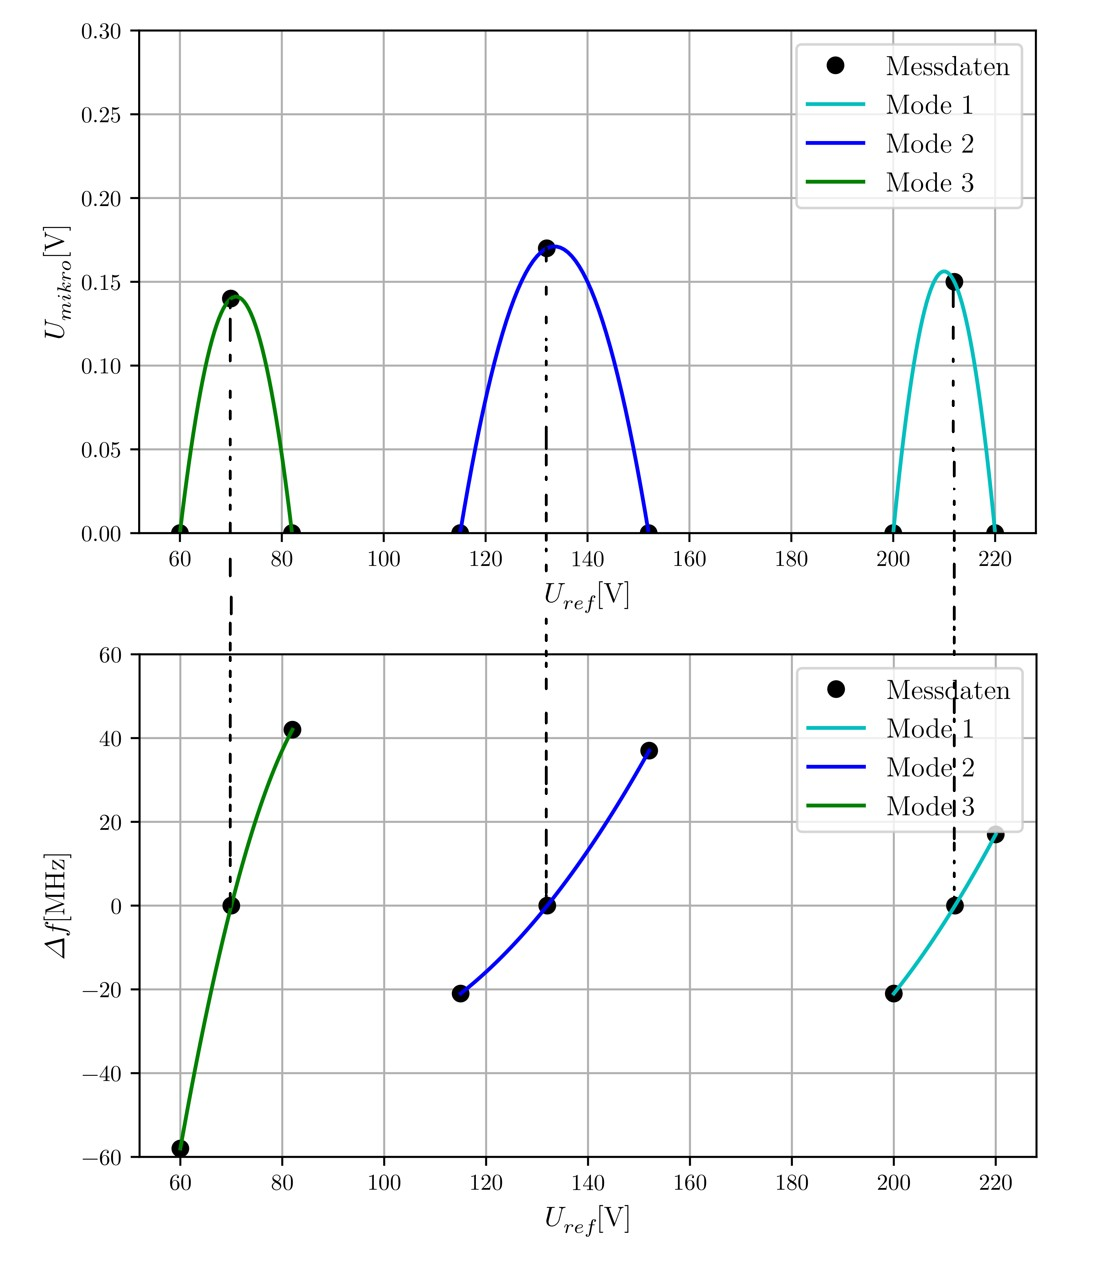
\includegraphics[width=0.8\textwidth]{bilder/SO.jpg}
    \label{fig:123}
    \caption{Der obere Graph stellt die parabelähnlichen, gefundenen Ausgleichsfunktionen zur Bestimmung der Detekorspannung dar. Die schwarzen
            Punkte sind die gefundenen Messwerte bei entsprechender Reflektorspannung $U_{ref}$ in Volt. Durch die gefundenen Parameter in \ref{tab:11}
            lässt sich so eine Funktion finden, die den Verlauf wiedergibt.    \\
            Analog für die Frequenzbestimmung formen die gefunden Parameter in \ref{tab:12} drei passende Ausgleichsfunktionenen in einem passenden 
            Intervall für die entsprechende Reflektorspannung $U_{ref}$. \\
            Durch eine vertikale Linie sind die Moden mit der zugehörigen Frequenzverschiebung verbunden.} 
    \label{fig:gimp}
\end{figure}

Die Abbildung \ref{fig:gimp} zeigt nun die Messwerte sowie die passenden Ausgleichspolynome. Diese lassen bereits auf die Bandbreite schließen. Um diese zu berechnen werden die um die Hälfte reduzierten maximalen Spannungen jeder Mode benötigt. Diese können
gemessen oder beispielsweise über die zuvor bestimmten Ausgleichsfunktionen genähert werden. Für die Bandbreite $B$ gilt ganz allgemein
\begin{equation}
    \label{eqn:g1}
B = f' - f''
\end{equation}
und die Abstimm-Empfindlichtkeit $A$ ist definiert als 
\begin{equation}
    \label{eqn:g2}
A = \frac{f' - f''}{V' - V''}.
\end{equation}
Dabei gibt $f'$ die halbe Maximumsfrequenz links vom Maximum und $f''$ rechts davon an. Das gleiche gilt für die Spannungen $V'$ und $V''$.
Die über die Funktionen genäherten Werte sind in der Tabelle \ref{tab:13} angegeben.
\begin{table}
    \centering
    \caption{Koeffizienten der Ausgleichspolynome der Frequenzshifts.} 
    \label{tab:13}
    \begin{tabular}{c || c c | c c}
        \toprule
        Mode &  $f'$ $[\si{\mega\hertz}] $& $f''$ $[\si{\mega\hertz}] $&  $V'$ $[\si{\volt}] $& $V''$ $[\si{\volt}] $ \\
        \midrule
        1      &      $\SI{9019.40}{}$      &       $\SI{9046.80}{}$              &        $\SI{202.79}{}$ &        $\SI{217.21}{}$ \\
        2      &      $\SI{9022.61}{}$      &       $\SI{9063.76}{}$              &        $\SI{120.38}{}$ &        $\SI{146.63}{}$ \\
        3      &      $\SI{9007.77}{}$      &       $\SI{9076.90}{}$              &        $\SI{63.19}{}$ &        $\SI{78.18}{}$ \\
    \end{tabular}
\end{table}
Aus diesen Werten lassen sich nun die Bandbreiten und Abstimm-Empfindlichtkeit leicht über die Gleichungen \ref{eqn:g1} und \ref{eqn:g2} berechnen. In der folgenden Tabelle \ref{tab:111} sind die Ergebnisse notiert.
\begin{table}
    \centering
    \caption{Bandbreiten und Abstimm-Empfindlichtkeiten.} 
    \label{tab:111}
    \begin{tabular}{c | c c}
        \toprule
        Mode &  Bandbreite $B$ $[\si{\mega\hertz}] $& Abstimm-Empfindlichtkeit $A$ $[\si{\mega\hertz\per\volt}]$ \\
        \midrule
        1      &      $\SI{27.40}{}$      &       $\SI{1.90}{}$              \\
        2      &      $\SI{41.15}{}$      &       $\SI{1.57}{}$              \\
        3      &      $\SI{69.13}{}$      &       $\SI{4.61}{}$               \\
    \end{tabular}
\end{table}

\subsection{Bestimmung von Frequenz, Wellenlänge und Dämpfung}

Aus den gemessenen Abständen zwischen den Minima der stehenden Wellen im Hohlleiter lässt sich die Wellenlänge im Hohlleiter $\lambda_h$ über
\begin{equation}
\increment x = \frac{\lambda_h}{2}
\end{equation}
berechnen. Mit den Messwerten aus Tabelle \ref{tab:Messreihe21} ergibt sich dadurch ein Wert von
\begin{equation}
\lambda_h = \SI{49}{\milli\meter}.
\end{equation}
Zusammen mit der Innenabmessung der längeren Seite des Hohlleiters
\begin{equation}
a = \SI{22.860(46)}{\milli\meter}
\end{equation}
lässt sich nun über die Gleichung \ref{eqn:222}, die Frequenz der longitudinalen Komponente berechnen.
Es ergibt sich 
\begin{equation}
f_h = \SI{8.968(10)}{\giga\hertz}.
\end{equation}
Über die klassische Beziehung 
\begin{equation}
v_{\text{phase}} = f_h \cdot \lambda_h
\end{equation}
lässt sich ebenfalls noch die Phasengeschwindigkeit bestimmen und es zeigt sich, dass mit 
\begin{equation}
v_{\text{phase}} = \left(\SI{1.4658(16)}{}\right) c
\end{equation}
die Phasengeschwindigkeit schneller als die Lichtgeschwindigkeit $c$ ist. Da diese allerdings, anders als die Gruppengeschwindigkeit, keine Informationen übertragt, ist dies nicht verwunderlich.
\\
\newline
Für die Bestimmung der Dämpfungskurve werden die gemessenen $\si{\decibel}$ und Gleitschraubentiefwerte aus der Tabelle \ref{tab:Messreihe22} in ein Diagramm geplottet.
Dafür wird wie zuvor ein Polynom zweiten Grades an die Theoriewerte gefittet. Die Form sieht wieder wie folgt aus
\begin{equation}
D = ax^2 + bx + c.
\end{equation}
Dabei steht das $D$ für die Dämpfung in $\si{\decibel}$ und die ermittelten Koeffizienten sind
\begin{align*}
a &= \SI{1.7014(1894)}{\decibel\per\milli\meter\squared}, \\
b &= \SI{0.4574(4478)}{\decibel\per\milli\meter}, \\
c &= \SI{0.0311(2385)}{\decibel}.
\end{align*}
Die gemessenen Werte, sowie das Ausgleichspolynom sind in der Abbildung \ref{111} zu erkennen.
\begin{figure}
    \centering
    \includegraphics[width=0.9\textwidth]{build/plot3.pdf}
    \caption{Abbildung zur Dämpfungskurve mit den gemessenen und Theoriewerten, sowie einem Ausgleichspolynom. Ergänzt wurden die korrigierten Messwerte.} 
    \label{111}
\end{figure}
Erkennbar ist der Offset zwischen den gemessenen und den theoretischen Werten, weshalb ebenfalls korrigierte Messwerte aufgetragen wurden. Diese werden in der Diskussion näher
erläutert.

\subsection{Stehwellenverhältnismessung}

\subsubsection{Direkte Methode}
Die Ergebnisse der direkten Methode sind in der Tabelle \ref{tab:Messreihe31} eingetragen. Sie dienen nachher als Vergleich zu den anderen Messmethoden.

\subsubsection{3 dB-Methode}
Alle Messungen zur 3 dB-Methode sind in der Tabelle \ref{tab:Messreihe32} aufgetragen. Hier wird wieder die Hohlleiterwellenlänge $\lambda_h$ 
benötigt welche wieder über die vorherige Methode der stehenden Welle zu
\begin{equation}
\lambda_h = 2 \cdot (\text{Min}_2 - \text{Min}_1) = \SI{47.60}{\milli\meter}
\end{equation}
bestimmt wird.
Über die Gleichung \ref{eqn:SWR} lässt sich nun ein Stehwellenverhältnis von
\begin{equation}
SWR = 8.987
\end{equation}
berechnen.

\subsubsection{Abschwächer-Methode}
Die für diese Methode nötigen Messwerte werden der Tabelle \label{tab:Messreihe33} entnommen.
$A_1$ und $A_2$ stehen für die gemessenen Dämpfungen bei den verschiedenen Einstellungen und führen mit der Gleichung 
\label{eqn:SWR2} zu dem Stehwellenverhältnis von
\begin{equation}
SWR = 14.125.
\end{equation}